\documentclass[]{article}
\usepackage{lmodern}
\usepackage{amssymb,amsmath}
\usepackage{ifxetex,ifluatex}
\usepackage{fixltx2e} % provides \textsubscript
\ifnum 0\ifxetex 1\fi\ifluatex 1\fi=0 % if pdftex
  \usepackage[T1]{fontenc}
  \usepackage[utf8]{inputenc}
\else % if luatex or xelatex
  \ifxetex
    \usepackage{mathspec}
    \usepackage{xltxtra,xunicode}
  \else
    \usepackage{fontspec}
  \fi
  \defaultfontfeatures{Mapping=tex-text,Scale=MatchLowercase}
  \newcommand{\euro}{€}
\fi
% use upquote if available, for straight quotes in verbatim environments
\IfFileExists{upquote.sty}{\usepackage{upquote}}{}
% use microtype if available
\IfFileExists{microtype.sty}{%
\usepackage{microtype}
\UseMicrotypeSet[protrusion]{basicmath} % disable protrusion for tt fonts
}{}
\usepackage[margin=1in]{geometry}
\usepackage{color}
\usepackage{fancyvrb}
\newcommand{\VerbBar}{|}
\newcommand{\VERB}{\Verb[commandchars=\\\{\}]}
\DefineVerbatimEnvironment{Highlighting}{Verbatim}{commandchars=\\\{\}}
% Add ',fontsize=\small' for more characters per line
\usepackage{framed}
\definecolor{shadecolor}{RGB}{248,248,248}
\newenvironment{Shaded}{\begin{snugshade}}{\end{snugshade}}
\newcommand{\KeywordTok}[1]{\textcolor[rgb]{0.13,0.29,0.53}{\textbf{{#1}}}}
\newcommand{\DataTypeTok}[1]{\textcolor[rgb]{0.13,0.29,0.53}{{#1}}}
\newcommand{\DecValTok}[1]{\textcolor[rgb]{0.00,0.00,0.81}{{#1}}}
\newcommand{\BaseNTok}[1]{\textcolor[rgb]{0.00,0.00,0.81}{{#1}}}
\newcommand{\FloatTok}[1]{\textcolor[rgb]{0.00,0.00,0.81}{{#1}}}
\newcommand{\CharTok}[1]{\textcolor[rgb]{0.31,0.60,0.02}{{#1}}}
\newcommand{\StringTok}[1]{\textcolor[rgb]{0.31,0.60,0.02}{{#1}}}
\newcommand{\CommentTok}[1]{\textcolor[rgb]{0.56,0.35,0.01}{\textit{{#1}}}}
\newcommand{\OtherTok}[1]{\textcolor[rgb]{0.56,0.35,0.01}{{#1}}}
\newcommand{\AlertTok}[1]{\textcolor[rgb]{0.94,0.16,0.16}{{#1}}}
\newcommand{\FunctionTok}[1]{\textcolor[rgb]{0.00,0.00,0.00}{{#1}}}
\newcommand{\RegionMarkerTok}[1]{{#1}}
\newcommand{\ErrorTok}[1]{\textbf{{#1}}}
\newcommand{\NormalTok}[1]{{#1}}
\usepackage{graphicx}
\makeatletter
\def\maxwidth{\ifdim\Gin@nat@width>\linewidth\linewidth\else\Gin@nat@width\fi}
\def\maxheight{\ifdim\Gin@nat@height>\textheight\textheight\else\Gin@nat@height\fi}
\makeatother
% Scale images if necessary, so that they will not overflow the page
% margins by default, and it is still possible to overwrite the defaults
% using explicit options in \includegraphics[width, height, ...]{}
\setkeys{Gin}{width=\maxwidth,height=\maxheight,keepaspectratio}
\ifxetex
  \usepackage[setpagesize=false, % page size defined by xetex
              unicode=false, % unicode breaks when used with xetex
              xetex]{hyperref}
\else
  \usepackage[unicode=true]{hyperref}
\fi
\hypersetup{breaklinks=true,
            bookmarks=true,
            pdfauthor={},
            pdftitle={Anaquin TransQuin Report},
            colorlinks=true,
            citecolor=blue,
            urlcolor=blue,
            linkcolor=magenta,
            pdfborder={0 0 0}}
\urlstyle{same}  % don't use monospace font for urls
\setlength{\parindent}{0pt}
\setlength{\parskip}{6pt plus 2pt minus 1pt}
\setlength{\emergencystretch}{3em}  % prevent overfull lines
\setcounter{secnumdepth}{0}

%%% Use protect on footnotes to avoid problems with footnotes in titles
\let\rmarkdownfootnote\footnote%
\def\footnote{\protect\rmarkdownfootnote}

%%% Change title format to be more compact
\usepackage{titling}

% Create subtitle command for use in maketitle
\newcommand{\subtitle}[1]{
  \posttitle{
    \begin{center}\large#1\end{center}
    }
}

\setlength{\droptitle}{-2em}
  \title{Anaquin TransQuin Report}
  \pretitle{\vspace{\droptitle}\centering\huge}
  \posttitle{\par}
  \author{}
  \preauthor{}\postauthor{}
  \date{}
  \predate{}\postdate{}

\usepackage{graphicx}


\begin{document}

\maketitle


\section{Read Alignment for accepted\_hits.bam
(A1)}\label{read-alignment-for-acceptedux5fhits.bam-a1}

\begin{Shaded}
\begin{Highlighting}[]
\NormalTok{Summary for dataset:}\StringTok{ }\NormalTok{A1/TransAlign_summary.stats}

   \NormalTok{Unmapped:}\StringTok{   }\DecValTok{0} \NormalTok{reads}
   \NormalTok{Experiment:}\StringTok{ }\DecValTok{6635268} \NormalTok{(}\FloatTok{21.5363}\NormalTok{%) reads}
   \NormalTok{Synthetic:}\StringTok{  }\DecValTok{24174356} \NormalTok{(}\FloatTok{78.4637}\NormalTok{%) reads}

   \NormalTok{Reference:}\StringTok{  }\DecValTok{1190} \NormalTok{exons}
   \NormalTok{Reference:}\StringTok{  }\DecValTok{1028} \NormalTok{introns}
   \NormalTok{Reference:}\StringTok{  }\DecValTok{149219} \NormalTok{bases}

   \NormalTok{Query:}\StringTok{      }\DecValTok{59421555} \NormalTok{exons}
   \NormalTok{Query:}\StringTok{      }\DecValTok{24855847} \NormalTok{introns}
   \NormalTok{Query:}\StringTok{      }\DecValTok{163383} \NormalTok{bases}

   \NormalTok{Dilution:}\StringTok{   }\FloatTok{0.784637}

   \NormalTok{**}\ErrorTok{*}
\StringTok{   }\ErrorTok{***}\StringTok{ }\NormalTok{The following statistics are computed at the exon, intron and base level.}
   \NormalTok{**}\ErrorTok{*}
\StringTok{   }\ErrorTok{***}\StringTok{ }\NormalTok{Exon level is defined by performance per exon. An alignment that}
   \NormalTok{**}\ErrorTok{*}\StringTok{ }\NormalTok{is not mapped entirely within an exon is considered as a FP. The}
   \NormalTok{**}\ErrorTok{*}\StringTok{ }\NormalTok{intron level is similar.}
   \NormalTok{**}\ErrorTok{*}
\StringTok{   }\ErrorTok{***}\StringTok{ }\NormalTok{Base level is defined by performance per nucleotide. A partial}
   \NormalTok{**}\ErrorTok{*}\StringTok{ }\NormalTok{mapped read will have FP and TP.}
   \NormalTok{**}\ErrorTok{*}

\StringTok{   }\NormalTok{--------------------}\StringTok{ }\NormalTok{Exon level --------------------}

\StringTok{   }\NormalTok{Sensitivity:}\StringTok{ }\FloatTok{0.994958}
   \NormalTok{Specificity:}\StringTok{ }\FloatTok{0.973343}
   \NormalTok{Detection:}\StringTok{   }\FloatTok{0.0590086} \NormalTok{(R2_33)}

   \NormalTok{--------------------}\StringTok{ }\NormalTok{Intron level --------------------}

\StringTok{   }\NormalTok{Sensitivity:}\StringTok{ }\FloatTok{0.991245}
   \NormalTok{Specificity:}\StringTok{ }\FloatTok{0.821653}
   \NormalTok{Detection:}\StringTok{   }\FloatTok{0.0590086} \NormalTok{(R2_33)}

   \NormalTok{--------------------}\StringTok{ }\NormalTok{Base level --------------------}

\StringTok{   }\NormalTok{Sensitivity:}\StringTok{ }\FloatTok{0.692468}
   \NormalTok{Specificity:}\StringTok{ }\FloatTok{0.924613}
   \NormalTok{Detection:}\StringTok{   }\FloatTok{0.0590086} \NormalTok{(R2_33)}

   \NormalTok{--------------------}\StringTok{ }\NormalTok{Undetected --------------------}

\StringTok{   }\NormalTok{Exon:}\StringTok{   }\FloatTok{0.005042}
   \NormalTok{Intron:}\StringTok{ }\FloatTok{0.008755}
   \NormalTok{Gene:}\StringTok{   }\FloatTok{0.052632}
\end{Highlighting}
\end{Shaded}

\pagebreak

\section{Read Alignment for accepted\_hits.bam
(A2)}\label{read-alignment-for-acceptedux5fhits.bam-a2}

\begin{Shaded}
\begin{Highlighting}[]
\NormalTok{Summary for dataset:}\StringTok{ }\NormalTok{A2/TransAlign_summary.stats}

   \NormalTok{Unmapped:}\StringTok{   }\DecValTok{0} \NormalTok{reads}
   \NormalTok{Experiment:}\StringTok{ }\DecValTok{5742035} \NormalTok{(}\FloatTok{20.4187}\NormalTok{%) reads}
   \NormalTok{Synthetic:}\StringTok{  }\DecValTok{22379420} \NormalTok{(}\FloatTok{79.5813}\NormalTok{%) reads}

   \NormalTok{Reference:}\StringTok{  }\DecValTok{1190} \NormalTok{exons}
   \NormalTok{Reference:}\StringTok{  }\DecValTok{1028} \NormalTok{introns}
   \NormalTok{Reference:}\StringTok{  }\DecValTok{149219} \NormalTok{bases}

   \NormalTok{Query:}\StringTok{      }\DecValTok{55184443} \NormalTok{exons}
   \NormalTok{Query:}\StringTok{      }\DecValTok{24887760} \NormalTok{introns}
   \NormalTok{Query:}\StringTok{      }\DecValTok{163986} \NormalTok{bases}

   \NormalTok{Dilution:}\StringTok{   }\FloatTok{0.795813}

   \NormalTok{**}\ErrorTok{*}
\StringTok{   }\ErrorTok{***}\StringTok{ }\NormalTok{The following statistics are computed at the exon, intron and base level.}
   \NormalTok{**}\ErrorTok{*}
\StringTok{   }\ErrorTok{***}\StringTok{ }\NormalTok{Exon level is defined by performance per exon. An alignment that}
   \NormalTok{**}\ErrorTok{*}\StringTok{ }\NormalTok{is not mapped entirely within an exon is considered as a FP. The}
   \NormalTok{**}\ErrorTok{*}\StringTok{ }\NormalTok{intron level is similar.}
   \NormalTok{**}\ErrorTok{*}
\StringTok{   }\ErrorTok{***}\StringTok{ }\NormalTok{Base level is defined by performance per nucleotide. A partial}
   \NormalTok{**}\ErrorTok{*}\StringTok{ }\NormalTok{mapped read will have FP and TP.}
   \NormalTok{**}\ErrorTok{*}

\StringTok{   }\NormalTok{--------------------}\StringTok{ }\NormalTok{Exon level --------------------}

\StringTok{   }\NormalTok{Sensitivity:}\StringTok{ }\FloatTok{0.996639}
   \NormalTok{Specificity:}\StringTok{ }\FloatTok{0.975178}
   \NormalTok{Detection:}\StringTok{   }\FloatTok{0.0590086} \NormalTok{(R2_33)}

   \NormalTok{--------------------}\StringTok{ }\NormalTok{Intron level --------------------}

\StringTok{   }\NormalTok{Sensitivity:}\StringTok{ }\FloatTok{0.991245}
   \NormalTok{Specificity:}\StringTok{ }\FloatTok{0.763722}
   \NormalTok{Detection:}\StringTok{   }\FloatTok{0.0590086} \NormalTok{(R2_33)}

   \NormalTok{--------------------}\StringTok{ }\NormalTok{Base level --------------------}

\StringTok{   }\NormalTok{Sensitivity:}\StringTok{ }\FloatTok{0.693059}
   \NormalTok{Specificity:}\StringTok{ }\FloatTok{0.921999}
   \NormalTok{Detection:}\StringTok{   }\FloatTok{0.0590086} \NormalTok{(R2_33)}

   \NormalTok{--------------------}\StringTok{ }\NormalTok{Undetected --------------------}

\StringTok{   }\NormalTok{Exon:}\StringTok{   }\FloatTok{0.003361}
   \NormalTok{Intron:}\StringTok{ }\FloatTok{0.008755}
   \NormalTok{Gene:}\StringTok{   }\FloatTok{0.039474}
\end{Highlighting}
\end{Shaded}

\pagebreak

\section{Read Alignment for accepted\_hits.bam
(A3)}\label{read-alignment-for-acceptedux5fhits.bam-a3}

\begin{Shaded}
\begin{Highlighting}[]
\NormalTok{Summary for dataset:}\StringTok{ }\NormalTok{A3/TransAlign_summary.stats}

   \NormalTok{Unmapped:}\StringTok{   }\DecValTok{0} \NormalTok{reads}
   \NormalTok{Experiment:}\StringTok{ }\DecValTok{5803436} \NormalTok{(}\FloatTok{21.0203}\NormalTok{%) reads}
   \NormalTok{Synthetic:}\StringTok{  }\DecValTok{21805238} \NormalTok{(}\FloatTok{78.9797}\NormalTok{%) reads}

   \NormalTok{Reference:}\StringTok{  }\DecValTok{1190} \NormalTok{exons}
   \NormalTok{Reference:}\StringTok{  }\DecValTok{1028} \NormalTok{introns}
   \NormalTok{Reference:}\StringTok{  }\DecValTok{149219} \NormalTok{bases}

   \NormalTok{Query:}\StringTok{      }\DecValTok{53748651} \NormalTok{exons}
   \NormalTok{Query:}\StringTok{      }\DecValTok{22830699} \NormalTok{introns}
   \NormalTok{Query:}\StringTok{      }\DecValTok{166153} \NormalTok{bases}

   \NormalTok{Dilution:}\StringTok{   }\FloatTok{0.789797}

   \NormalTok{**}\ErrorTok{*}
\StringTok{   }\ErrorTok{***}\StringTok{ }\NormalTok{The following statistics are computed at the exon, intron and base level.}
   \NormalTok{**}\ErrorTok{*}
\StringTok{   }\ErrorTok{***}\StringTok{ }\NormalTok{Exon level is defined by performance per exon. An alignment that}
   \NormalTok{**}\ErrorTok{*}\StringTok{ }\NormalTok{is not mapped entirely within an exon is considered as a FP. The}
   \NormalTok{**}\ErrorTok{*}\StringTok{ }\NormalTok{intron level is similar.}
   \NormalTok{**}\ErrorTok{*}
\StringTok{   }\ErrorTok{***}\StringTok{ }\NormalTok{Base level is defined by performance per nucleotide. A partial}
   \NormalTok{**}\ErrorTok{*}\StringTok{ }\NormalTok{mapped read will have FP and TP.}
   \NormalTok{**}\ErrorTok{*}

\StringTok{   }\NormalTok{--------------------}\StringTok{ }\NormalTok{Exon level --------------------}

\StringTok{   }\NormalTok{Sensitivity:}\StringTok{ }\FloatTok{0.996639}
   \NormalTok{Specificity:}\StringTok{ }\FloatTok{0.974466}
   \NormalTok{Detection:}\StringTok{   }\FloatTok{0.0590086} \NormalTok{(R2_33)}

   \NormalTok{--------------------}\StringTok{ }\NormalTok{Intron level --------------------}

\StringTok{   }\NormalTok{Sensitivity:}\StringTok{ }\FloatTok{0.992218}
   \NormalTok{Specificity:}\StringTok{ }\FloatTok{0.811167}
   \NormalTok{Detection:}\StringTok{   }\FloatTok{0.0590086} \NormalTok{(R2_33)}

   \NormalTok{--------------------}\StringTok{ }\NormalTok{Base level --------------------}

\StringTok{   }\NormalTok{Sensitivity:}\StringTok{ }\FloatTok{0.695741}
   \NormalTok{Specificity:}\StringTok{ }\FloatTok{0.913495}
   \NormalTok{Detection:}\StringTok{   }\FloatTok{0.0590086} \NormalTok{(R2_33)}

   \NormalTok{--------------------}\StringTok{ }\NormalTok{Undetected --------------------}

\StringTok{   }\NormalTok{Exon:}\StringTok{   }\FloatTok{0.003361}
   \NormalTok{Intron:}\StringTok{ }\FloatTok{0.007782}
   \NormalTok{Gene:}\StringTok{   }\FloatTok{0.039474}
\end{Highlighting}
\end{Shaded}

\pagebreak

\section{Read Alignment for accepted\_hits.bam
(B1)}\label{read-alignment-for-acceptedux5fhits.bam-b1}

\begin{Shaded}
\begin{Highlighting}[]
\NormalTok{Summary for dataset:}\StringTok{ }\NormalTok{B1/TransAlign_summary.stats}

   \NormalTok{Unmapped:}\StringTok{   }\DecValTok{0} \NormalTok{reads}
   \NormalTok{Experiment:}\StringTok{ }\DecValTok{3564555} \NormalTok{(}\FloatTok{14.1897}\NormalTok{%) reads}
   \NormalTok{Synthetic:}\StringTok{  }\DecValTok{21556180} \NormalTok{(}\FloatTok{85.8103}\NormalTok{%) reads}

   \NormalTok{Reference:}\StringTok{  }\DecValTok{1190} \NormalTok{exons}
   \NormalTok{Reference:}\StringTok{  }\DecValTok{1028} \NormalTok{introns}
   \NormalTok{Reference:}\StringTok{  }\DecValTok{149219} \NormalTok{bases}

   \NormalTok{Query:}\StringTok{      }\DecValTok{57069428} \NormalTok{exons}
   \NormalTok{Query:}\StringTok{      }\DecValTok{26914113} \NormalTok{introns}
   \NormalTok{Query:}\StringTok{      }\DecValTok{158601} \NormalTok{bases}

   \NormalTok{Dilution:}\StringTok{   }\FloatTok{0.858103}

   \NormalTok{**}\ErrorTok{*}
\StringTok{   }\ErrorTok{***}\StringTok{ }\NormalTok{The following statistics are computed at the exon, intron and base level.}
   \NormalTok{**}\ErrorTok{*}
\StringTok{   }\ErrorTok{***}\StringTok{ }\NormalTok{Exon level is defined by performance per exon. An alignment that}
   \NormalTok{**}\ErrorTok{*}\StringTok{ }\NormalTok{is not mapped entirely within an exon is considered as a FP. The}
   \NormalTok{**}\ErrorTok{*}\StringTok{ }\NormalTok{intron level is similar.}
   \NormalTok{**}\ErrorTok{*}
\StringTok{   }\ErrorTok{***}\StringTok{ }\NormalTok{Base level is defined by performance per nucleotide. A partial}
   \NormalTok{**}\ErrorTok{*}\StringTok{ }\NormalTok{mapped read will have FP and TP.}
   \NormalTok{**}\ErrorTok{*}

\StringTok{   }\NormalTok{--------------------}\StringTok{ }\NormalTok{Exon level --------------------}

\StringTok{   }\NormalTok{Sensitivity:}\StringTok{ }\FloatTok{0.992437}
   \NormalTok{Specificity:}\StringTok{ }\FloatTok{0.981463}
   \NormalTok{Detection:}\StringTok{   }\FloatTok{0.0590086} \NormalTok{(R2_33)}

   \NormalTok{--------------------}\StringTok{ }\NormalTok{Intron level --------------------}

\StringTok{   }\NormalTok{Sensitivity:}\StringTok{ }\FloatTok{0.986381}
   \NormalTok{Specificity:}\StringTok{ }\FloatTok{0.880564}
   \NormalTok{Detection:}\StringTok{   }\FloatTok{1.88828} \NormalTok{(R1_72)}

   \NormalTok{--------------------}\StringTok{ }\NormalTok{Base level --------------------}

\StringTok{   }\NormalTok{Sensitivity:}\StringTok{ }\FloatTok{0.685079}
   \NormalTok{Specificity:}\StringTok{ }\FloatTok{0.942327}
   \NormalTok{Detection:}\StringTok{   }\FloatTok{0.0590086} \NormalTok{(R2_33)}

   \NormalTok{--------------------}\StringTok{ }\NormalTok{Undetected --------------------}

\StringTok{   }\NormalTok{Exon:}\StringTok{   }\FloatTok{0.007563}
   \NormalTok{Intron:}\StringTok{ }\FloatTok{0.013619}
   \NormalTok{Gene:}\StringTok{   }\FloatTok{0.065789}
\end{Highlighting}
\end{Shaded}

\pagebreak

\section{Read Alignment for accepted\_hits.bam
(B2)}\label{read-alignment-for-acceptedux5fhits.bam-b2}

\begin{Shaded}
\begin{Highlighting}[]
\NormalTok{Summary for dataset:}\StringTok{ }\NormalTok{B2/TransAlign_summary.stats}

   \NormalTok{Unmapped:}\StringTok{   }\DecValTok{0} \NormalTok{reads}
   \NormalTok{Experiment:}\StringTok{ }\DecValTok{3673262} \NormalTok{(}\FloatTok{14.5259}\NormalTok{%) reads}
   \NormalTok{Synthetic:}\StringTok{  }\DecValTok{21614486} \NormalTok{(}\FloatTok{85.4741}\NormalTok{%) reads}

   \NormalTok{Reference:}\StringTok{  }\DecValTok{1190} \NormalTok{exons}
   \NormalTok{Reference:}\StringTok{  }\DecValTok{1028} \NormalTok{introns}
   \NormalTok{Reference:}\StringTok{  }\DecValTok{149219} \NormalTok{bases}

   \NormalTok{Query:}\StringTok{      }\DecValTok{57264502} \NormalTok{exons}
   \NormalTok{Query:}\StringTok{      }\DecValTok{28885125} \NormalTok{introns}
   \NormalTok{Query:}\StringTok{      }\DecValTok{160649} \NormalTok{bases}

   \NormalTok{Dilution:}\StringTok{   }\FloatTok{0.854741}

   \NormalTok{**}\ErrorTok{*}
\StringTok{   }\ErrorTok{***}\StringTok{ }\NormalTok{The following statistics are computed at the exon, intron and base level.}
   \NormalTok{**}\ErrorTok{*}
\StringTok{   }\ErrorTok{***}\StringTok{ }\NormalTok{Exon level is defined by performance per exon. An alignment that}
   \NormalTok{**}\ErrorTok{*}\StringTok{ }\NormalTok{is not mapped entirely within an exon is considered as a FP. The}
   \NormalTok{**}\ErrorTok{*}\StringTok{ }\NormalTok{intron level is similar.}
   \NormalTok{**}\ErrorTok{*}
\StringTok{   }\ErrorTok{***}\StringTok{ }\NormalTok{Base level is defined by performance per nucleotide. A partial}
   \NormalTok{**}\ErrorTok{*}\StringTok{ }\NormalTok{mapped read will have FP and TP.}
   \NormalTok{**}\ErrorTok{*}

\StringTok{   }\NormalTok{--------------------}\StringTok{ }\NormalTok{Exon level --------------------}

\StringTok{   }\NormalTok{Sensitivity:}\StringTok{ }\FloatTok{0.994118}
   \NormalTok{Specificity:}\StringTok{ }\FloatTok{0.981653}
   \NormalTok{Detection:}\StringTok{   }\FloatTok{0.0590086} \NormalTok{(R2_33)}

   \NormalTok{--------------------}\StringTok{ }\NormalTok{Intron level --------------------}

\StringTok{   }\NormalTok{Sensitivity:}\StringTok{ }\FloatTok{0.984436}
   \NormalTok{Specificity:}\StringTok{ }\FloatTok{0.818059}
   \NormalTok{Detection:}\StringTok{   }\FloatTok{0.0590086} \NormalTok{(R2_33)}

   \NormalTok{--------------------}\StringTok{ }\NormalTok{Base level --------------------}

\StringTok{   }\NormalTok{Sensitivity:}\StringTok{ }\FloatTok{0.687879}
   \NormalTok{Specificity:}\StringTok{ }\FloatTok{0.934117}
   \NormalTok{Detection:}\StringTok{   }\FloatTok{0.0590086} \NormalTok{(R2_33)}

   \NormalTok{--------------------}\StringTok{ }\NormalTok{Undetected --------------------}

\StringTok{   }\NormalTok{Exon:}\StringTok{   }\FloatTok{0.005882}
   \NormalTok{Intron:}\StringTok{ }\FloatTok{0.015564}
   \NormalTok{Gene:}\StringTok{   }\FloatTok{0.052632}
\end{Highlighting}
\end{Shaded}

\pagebreak

\section{Read Alignment for accepted\_hits.bam
(B3)}\label{read-alignment-for-acceptedux5fhits.bam-b3}

\begin{Shaded}
\begin{Highlighting}[]
\NormalTok{Summary for dataset:}\StringTok{ }\NormalTok{B3/TransAlign_summary.stats}

   \NormalTok{Unmapped:}\StringTok{   }\DecValTok{0} \NormalTok{reads}
   \NormalTok{Experiment:}\StringTok{ }\DecValTok{4705904} \NormalTok{(}\FloatTok{15.6992}\NormalTok{%) reads}
   \NormalTok{Synthetic:}\StringTok{  }\DecValTok{25269549} \NormalTok{(}\FloatTok{84.3008}\NormalTok{%) reads}

   \NormalTok{Reference:}\StringTok{  }\DecValTok{1190} \NormalTok{exons}
   \NormalTok{Reference:}\StringTok{  }\DecValTok{1028} \NormalTok{introns}
   \NormalTok{Reference:}\StringTok{  }\DecValTok{149219} \NormalTok{bases}

   \NormalTok{Query:}\StringTok{      }\DecValTok{67685272} \NormalTok{exons}
   \NormalTok{Query:}\StringTok{      }\DecValTok{37139930} \NormalTok{introns}
   \NormalTok{Query:}\StringTok{      }\DecValTok{162712} \NormalTok{bases}

   \NormalTok{Dilution:}\StringTok{   }\FloatTok{0.843008}

   \NormalTok{**}\ErrorTok{*}
\StringTok{   }\ErrorTok{***}\StringTok{ }\NormalTok{The following statistics are computed at the exon, intron and base level.}
   \NormalTok{**}\ErrorTok{*}
\StringTok{   }\ErrorTok{***}\StringTok{ }\NormalTok{Exon level is defined by performance per exon. An alignment that}
   \NormalTok{**}\ErrorTok{*}\StringTok{ }\NormalTok{is not mapped entirely within an exon is considered as a FP. The}
   \NormalTok{**}\ErrorTok{*}\StringTok{ }\NormalTok{intron level is similar.}
   \NormalTok{**}\ErrorTok{*}
\StringTok{   }\ErrorTok{***}\StringTok{ }\NormalTok{Base level is defined by performance per nucleotide. A partial}
   \NormalTok{**}\ErrorTok{*}\StringTok{ }\NormalTok{mapped read will have FP and TP.}
   \NormalTok{**}\ErrorTok{*}

\StringTok{   }\NormalTok{--------------------}\StringTok{ }\NormalTok{Exon level --------------------}

\StringTok{   }\NormalTok{Sensitivity:}\StringTok{ }\FloatTok{0.994958}
   \NormalTok{Specificity:}\StringTok{ }\FloatTok{0.980831}
   \NormalTok{Detection:}\StringTok{   }\FloatTok{0.0590086} \NormalTok{(R2_33)}

   \NormalTok{--------------------}\StringTok{ }\NormalTok{Intron level --------------------}

\StringTok{   }\NormalTok{Sensitivity:}\StringTok{ }\FloatTok{0.986381}
   \NormalTok{Specificity:}\StringTok{ }\FloatTok{0.759454}
   \NormalTok{Detection:}\StringTok{   }\FloatTok{0.0590086} \NormalTok{(R2_33)}

   \NormalTok{--------------------}\StringTok{ }\NormalTok{Base level --------------------}

\StringTok{   }\NormalTok{Sensitivity:}\StringTok{ }\FloatTok{0.688292}
   \NormalTok{Specificity:}\StringTok{ }\FloatTok{0.922827}
   \NormalTok{Detection:}\StringTok{   }\FloatTok{0.0590086} \NormalTok{(R2_33)}

   \NormalTok{--------------------}\StringTok{ }\NormalTok{Undetected --------------------}

\StringTok{   }\NormalTok{Exon:}\StringTok{   }\FloatTok{0.005042}
   \NormalTok{Intron:}\StringTok{ }\FloatTok{0.013619}
   \NormalTok{Gene:}\StringTok{   }\FloatTok{0.052632}
\end{Highlighting}
\end{Shaded}

\pagebreak

\begin{verbatim}
Summary for dataset: /Users/tedwong/Desktop/K_562/Cuffdiffs/gene_exp.diff

   Experiment:  9682 genes
   Synthetic:   67 genes

   Reference:   76 genes
   Detected:    65 genes

   ***
   *** Statistics for linear regression
   ***

   Correlation: 0.56272
   Slope:       0.411349
   R2:          0.316654
   F-statistic: 29.1934
   P-value:     1.06667e-06
   SSM:         244.21, DF: 1
   SSE:         527.011, DF: 63
   SST:         771.221, DF: 64

   ***
   *** Statistics for linear regression (log2 scale)
   ***

   Correlation: 0.769414
   Slope:       0.545994
   R2:          0.591998
   F-statistic: 91.4108
   P-value:     7.00551e-14
   SSM:         116.382, DF: 1
   SSE:         80.21, DF: 63
   SST:         196.592, DF: 64
\end{verbatim}

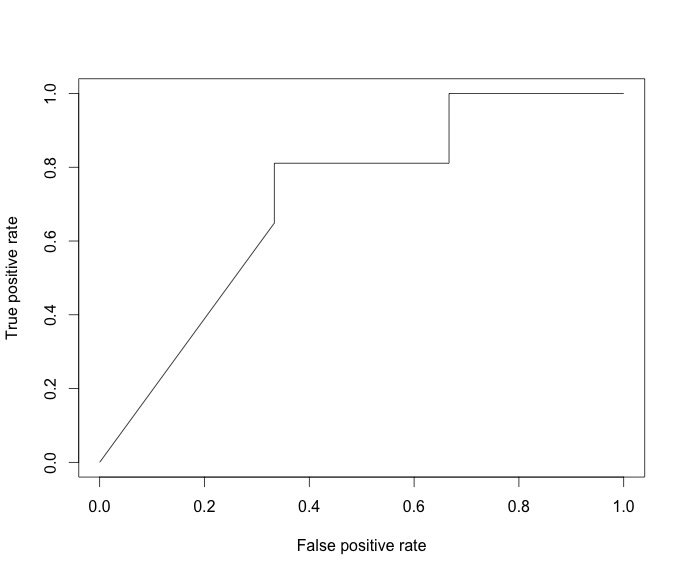
\includegraphics{samples/ROCSample.jpeg}
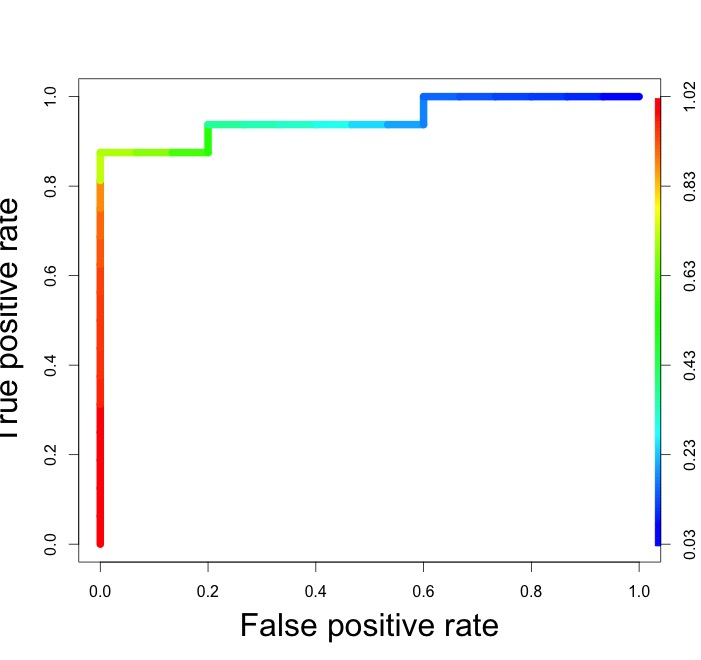
\includegraphics{samples/ROCSampleColour.jpeg}
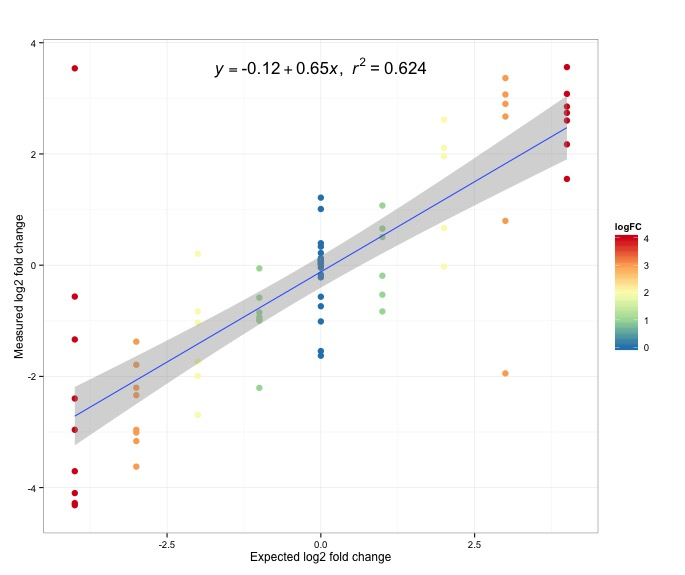
\includegraphics{samples/ScatterLFCSample.jpeg}
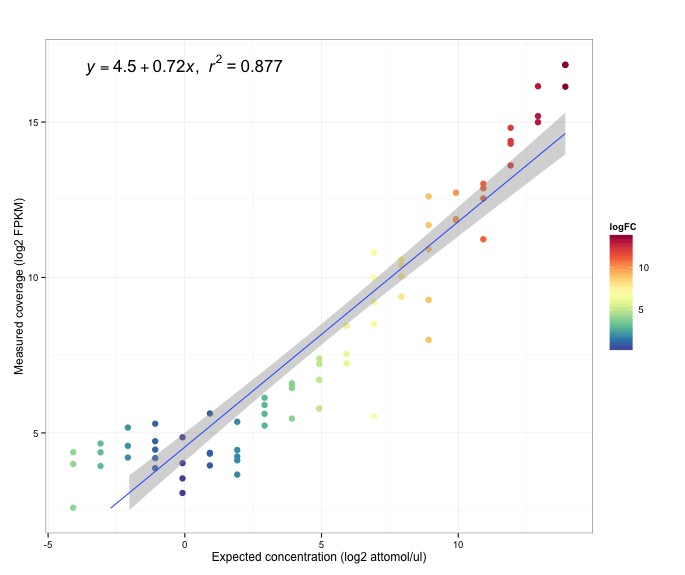
\includegraphics{samples/TransExpress_Sample.jpeg}

\pagebreak

\begin{verbatim}
Summary for dataset: /Users/tedwong/Desktop/K_562/Cufflinks/A1/genes.fpkm_tracking

   Experiment:  60570 gene
   Synthetic:   75 gene

   Reference:   76 gene
   Detected:    4.39067 gene

   ***
   *** Detection Limits
   ***

   Break: 3.77655 (R1_62)

   Left:  4.39067 + 0.0805742x (R2 = 0.0567335)
   Right: 2.0794 + 1.00352x (R2 = 0.922502)

   ***
   *** Statistics for linear regression
   ***

   Correlation: 0.962825
   Slope:       6.46625
   R2:          0.927032
   F-statistic: 902.032
   P-value:     0
   SSM:         3.50824e+10, DF: 1
   SSE:         2.76138e+09, DF: 71
   SST:         3.78438e+10, DF: 72

   ***
   *** Statistics for linear regression (log2 scale)
   ***

   Correlation: 0.936306
   Slope:       0.724913
   R2:          0.876669
   F-statistic: 504.686
   P-value:     0
   SSM:         1040.46, DF: 1
   SSE:         146.373, DF: 71
   SST:         1186.83, DF: 72
\end{verbatim}

\end{document}
